\documentclass[
	% -- opções da classe memoir --
	11pt,				% tamanho da fonte
	openright,			% capítulos começam em pág ímpar (insere página vazia caso preciso)
	twoside,			% para impressão em recto e verso. Oposto a oneside
	a5paper,			% tamanho do papel. 
	% -- opções da classe abntex2 --
	%chapter=TITLE,		% títulos de capítulos convertidos em letras maiúsculas
	%section=TITLE,		% títulos de seções convertidos em letras maiúsculas
	%subsection=TITLE,	% títulos de subseções convertidos em letras maiúsculas
	%subsubsection=TITLE,% títulos de subsubseções convertidos em letras maiúsculas
	% -- opções do pacote babel --
	english,			% idioma adicional para hifenização
	french,				% idioma adicional para hifenização
	spanish,			% idioma adicional para hifenização
	brazil,				% o último idioma é o principal do documento
	sumario=tradicional
]{abntex2}

% compilação de fontes

\usepackage{ifxetex}
\ifxetex
  % % se for utilizar as fontes do sistema: **escolha sua fonte**
  \usepackage{polyglossia}
  \setmainlanguage{brazil}
  \setotherlanguages{french,english,spanish,german,italian}
  \usepackage{fontspec}
  \defaultfontfeatures{Ligatures=TeX}
  % comandos de fontes
  \setmainfont[Numbers=OldStyle]{Minion Pro} %fonte principal (serifada)
  \setsansfont[Scale=0.9]{Myriad Pro} %fonte sem serifas
  \setmonofont[Scale=MatchLowercase]{Consolas} % fonte monoespaçada
\else
  % % se for utilizar pdflatex
  \usepackage[utf8]{inputenc}
  \usepackage[T1]{fontenc}
  \usepackage{fourier}
  \usepackage[defaultsans]{droidsans} %fonte droid sans como default sans, ao invés de CM Sans.
  \usepackage[scaled=0.9]{inconsolata} %fonte inconsolata para códigos
  \usepackage[defaultmono,scale=0.8]{droidmono} %fonte droid mono para códigos
\fi

%% Observação: o pacote polyglossia pode apresentar erro ao ser utilizado com ifxetex + babel. 
%% Se isso acontecer, atualize o pacote para a versão mais recente ou utilize somente uma das sequências (pdflatex ou xelatex), comentando ou apagando a outra.

\usepackage{microtype} 				% para melhorias de justificação
\usepackage[usenames,dvipsnames]{xcolor} 	% para cores
\usepackage{graphicx} 				% para imagens
\usepackage{booktabs,tabularx,rotating}% para tabelas
\usepackage{mdframed} 				% para caixas de texto como na CIP do verso do título
\usepackage{multicol}				% tabelas com colunas mescladas
\usepackage{lettrine}				% letras capitulares
\usepackage{xspace} 				% para nao precisar de espaços com {} depois de comandos
									% como \LaTeX e abreviações criadas pelo usuário
\usepackage{lipsum} 				% para texto de preenchimento de exemplo
\usepackage{leading}				% espaçamento entrelinhas (leading)
\leading{13pt}

%\newcommand{\textbsf}[1]{\textbf{\textsf{#1}}

% ---
% Pacotes de citações
% ---
\usepackage[brazilian,hyperpageref]{backref}	 % Paginas com as citações na bibl
\usepackage[alf]{abntex2cite}	% Citações padrão ABNT

% ---
% Inclusão de códigos de LP
% ---
\usepackage{listings}
\lstset{
  language=C++,
  basicstyle=\ttfamily\footnotesize, 
  keywordstyle=\color{blue}, 
  stringstyle=\color{x}, 
  commentstyle=\color{red}, 
  extendedchars=true, 
  showspaces=false, 
  showstringspaces=false, 
  %numbers=left,
 % numberstyle=\tiny,
  breaklines=true, 
  backgroundcolor=\color{gray!10},
  breakautoindent=true, 
  captionpos=t,
  xleftmargin=0pt,
}

% ---
% BOX ARREDONDADO http://texdoc.net/texmf-dist/doc/latex/tcolorbox/tcolorbox.pdf
% ---
\usepackage{tcolorbox}

% ---
% CAPA
% ---
\usepackage{pstricks}
\usepackage{mathptmx}
\usepackage{anyfontsize}
\usepackage{emerald}
\usepackage[T1]{fontenc}
\usepackage{t1enc}
\definecolor{grafitte}{rgb}{0.266,0.258,0.258}
\definecolor{gray}{rgb}{0.529,0.525,0.541}
\definecolor{verde}{rgb}{0.329,0.925,0.541}
\definecolor{mostarda}{rgb}{0.900,0.900,0.241}
\definecolor{x}{rgb}{0.900,0.500,0.120}



\usepackage[referable]{threeparttablex}

% ---
% CONTRA-CAPA
% ---

\newcommand{\plogo}{\fbox{$\mathcal{UFLA}$}} % Generic dummy publisher logo

\usepackage[T1]{fontenc} % Output font encoding for international characters
\usepackage{fouriernc} % Use the New Century Schoolbook font

% ---
% Graficos
% ---
\usepackage{tikz}
\usepackage{pgfplots}

% ---
% Tabelas
% ---
\usepackage{tcolorbox}
\usepackage{tabularx}
\usepackage{array}
\usepackage{colortbl}
\tcbuselibrary{skins}

\newcolumntype{Y}{>{\raggedleft\arraybackslash}X}

\tcbset{tab2/.style={enhanced,fonttitle=\bfseries,fontupper=\normalsize\sffamily,
colback=blue!10!white,colframe=red!50!black,colbacktitle=Salmon!40!white,
coltitle=black,center title}}



% ---
% Configurações do pacote backref
% Usado sem a opção hyperpageref de backref
\renewcommand{\backrefpagesname}{Citado na(s) página(s):~}
% Texto padrão antes do número das páginas
\renewcommand{\backref}{}
% Define os textos da citação
\renewcommand*{\backrefalt}[4]{
	\ifcase #1 %
		Nenhuma citação no texto.%
	\or
		Citado na página #2.%
	\else
		Citado #1 vezes nas páginas #2.%
	\fi}%
% ---

% ---
% Informações do documento
% ---
\titulo{ESP8266 - Uma Introdução ao Desenvolvimento em IoT}
\autor{Gabriel M. de Melo}
\data{2017, v-1.0}
\preambulo{Breve sinopse do livro}
\local{Lavras-MG}
\instituicao{Universidade Federal de Lavras}

% alterando o aspecto da cor azul
\definecolor{blue}{RGB}{41,5,195}

% informações do PDF
\makeatletter
\hypersetup{
     	%pagebackref=true,
		pdftitle={\@title}, 
		pdfauthor={\@author},
    	pdfsubject={\imprimirpreambulo},
	    pdfcreator={LaTeX with abnTeX2},
		pdfkeywords={abnt}{latex}{abntex}{abntex2}{livro}, 
		colorlinks=true,       		% false: boxed links; true: colored links
    	linkcolor=blue,          	% color of internal links
    	citecolor=blue,        		% color of links to bibliography
    	filecolor=magenta,      		% color of file links
		urlcolor=blue,
		bookmarksdepth=4
}
\makeatother
% ---


% ---
% Estilo de capítulos
%
% \chapterstyle{pedersen} 
%\chapterstyle{lyhne} 
%\chapterstyle{madsen} 
\chapterstyle{veelo} 
%
% Veja outros estilos em:
% https://www.ctan.org/tex-archive/info/MemoirChapStyles
% ---

% para cabeçalhos sem estar em maiúsculas
%\nouppercaseheads 

% -----
% Declarações de cabecalhos 
% -----
% Cabecalho padrao
\makepagestyle{abntbookheadings}
\makeevenhead{abntbookheadings}{\ABNTEXfontereduzida\thepage}{}{\ABNTEXfontereduzida\textit\leftmark}
\makeoddhead{abntbookheadings}{\ABNTEXfontereduzida\textit\rightmark}{}{\ABNTEXfontereduzida\thepage}
\makeheadrule{abntbookheadings}{\textwidth}{\normalrulethickness}

% Cabecalho do inicio do capitulo
\makepagestyle{abntbookchapfirst}
\makeoddhead{abntbookchapfirst}{}{}{}

% Configura layout para elementos textuais
\renewcommand{\textual}{%
  \pagestyle{abntbookheadings}%
  \aliaspagestyle{chapter}{abntbookchapfirst}% customizing chapter pagestyle
  \nouppercaseheads%
  \bookmarksetup{startatroot}% 
}
% ---

% ---
% Espaçamentos entre linhas e parágrafos
% ---
% O tamanho do parágrafo é dado por (exemplo):
%\setlength{\parindent}{1.3cm}
%% Não recomendado mudar.
 
% Controle do espaçamento entre um parágrafo e outro:
%\setlength{\parskip}{0.2cm}  % tente também \onelineskip
%% Não recomendado mudar.

% Margens do documento 
%% (margens do abntex2 não combinam nem com A5 nem com estilos de capítulo da
% classe memoir.)
\setlrmarginsandblock{2.5cm}{3.5cm}{*}
\setulmarginsandblock{2.5cm}{3.5cm}{*}
\checkandfixthelayout
% ---

% ---
% Início do documento
% ---
\begin{document}

% ---
% Capa principal
% ---
%\noindent
%%\begin{pspicture}(0,17.5)(\linewidth,0)
%  \psline[linewidth=6mm,linecolor=grafitte](-2.74,19.7)(10.50,19.7)
  %\rput(\linewidth,17.5)
   % {\pspolygon*(1.5,4.45)(3.7,4.45)(4.8,3.45)(4.8,1.25)}
 % \rput(\linewidth,17.5)
 %   {\rput{-45}(-1,-1){\Large\textbf{\white Primeira}}}
 % \rput(\linewidth,17.5)
 %   {\rput{-45}(-1.5,-1.5){\Large\textbf{\white edição}}}
%desenho    
%  {\pspolygon*(-5.74,-6)(-4.7,-1)(16.86,-1)(16.86,-6)}
 % {\pspolygon*[linecolor=grafitte](-5.74, 15)(-4.7,7)(16.86,7)(16.86,15)}
  
  %\rput[l](-2.74,12.7){\textsl{ \textbf{\fontsize{90}{90}\selectfont \ECFAugie \white O}}}
  %\rput[l](0,12.5){\textsl{ \textbf{\fontsize{70}{90}\selectfont \ECFAugie \white ESP8266}}}
  %\psline[linewidth=2mm,linecolor=white](-2.74,10.8)(10.50,10.8)
  %\rput[l](-2.74,9.8){\textsl{ \ECFAugie \fontsize{30}{90}\selectfont \white Uma introducao \`a}}
  %\rput[l](-2.74,8.8){\textsl{ \ECFAugie \fontsize{30}{90}\selectfont \white  Internet das Coisas}}
 % 
  %\psline[linewidth=3mm,linecolor=gray](-5.74,15)(16.86,15)
  %\psline[linewidth=3mm,linecolor=gray](-5.74,7)(16.86,7)
    
 % \rput[l](-2,7){\textsl{ \textbf{\fontsize{50}{50}\selectfont \ECFAugie Internet das Coisas}}}
  %\rput[l](2,6){\psscaleboxto(\textwidth,0.9){ \emph{Gabriel M. de Melo}}}
  
%\end{pspicture}

% ---
% Capa principal 2
% ---




\frenchspacing

\frontmatter

% ---
% Capa principal
% ---
%\begin{titlingpage}
%\phantom{xxx}
%\vspace{0.5cm}
%\huge
%\raggedright
%\imprimirautor\\
%\vspace{2.5cm}
%\huge 
%{\raggedleft
%\includegraphics[scale=0.9]{abntex2-modelo-img-marca.pdf}\\[1cm]
%\textit{\textcolor{black}{ \textsf{\textbf{\imprimirtitulo}}}}\\[1cm]
%}
%\centering 
%%  %este é um símbolo que só aparecerá com a fonte Minion.
%\vfill
%\Large
% %este é um símbolo que só aparecerá com a fonte Minion.
%\hspace{20pt} \imprimirinstituicao
%\end{titlingpage}
% ---

% ---
% Contra-capa
% ---
\begin{titlingpage} % Suppresses headers and footers on the title page
	
	\centering % Centre everything on the title page
	
	%------------------------------------------------
	%	Top rules
	%------------------------------------------------
	
	\rule{270pt}{1pt} % Thick horizontal rule
	
	\vspace{2pt}\vspace{-\baselineskip} % Whitespace between rules
	
	\rule{270pt}{0.4pt} % Thin horizontal rule
	
	\vspace{0.1\textheight} % Whitespace between the top rules and title
	
	%------------------------------------------------
	%	Title
	%------------------------------------------------
	
	\textcolor{Black!80}{
	\centering% Red font color
	\hspace{10pt}	{\Huge O ESP8266}\\[0.5\baselineskip] % Title line 1
	\hspace{10pt}	{\Large Uma introdução à Internet das Coisas}\\[0.5\baselineskip] % Title line 2
	%	{\Large  Internet das Coisas} % Title line 3
	}
	
	\vspace{0.025\textheight} % Whitespace between the title and short horizontal rule
	
%	\rule{0.3\textwidth}{0.4pt} % Short horizontal rule under the title
	
	\vspace{0.1\textheight} % Whitespace between the thin horizontal rule and the author name
	
	%------------------------------------------------
	%	Author
	%------------------------------------------------
	
	\hspace{10pt}{\Large \textsc{Gabriel M. Melo}} % Author name
	
	\vfill % Whitespace between the author name and publisher
	
	%------------------------------------------------
	%	Publisher
	%------------------------------------------------
	\hspace{10pt}{\Large{\textsc{EMakers}}}
	\vspace{10pt}
	
	\hspace{10pt}\textsc{Núcleo de estudos em Sistemas Embarcados, Internet das Coisas e Otimização}
	
	UFLA
	
    %{\centering
	%\begin{figure}[ht]
    %\centering
    %\hspace{10pt}
\includegraphics[scale=0.9]{logo_Oficial.png}
    %%\caption{Caption}
    %\label{fig:my_label}
    %\end{figure}
	%{\large\textcolor{Gray}{\plogo}}\\[0.5\baselineskip] % Publisher logo
	%}
	%{\large\textsc{the publisher}} % Publisher
	
	\vspace{0.1\textheight} % Whitespace under the publisher text
	
	%------------------------------------------------
	%	Bottom rules
	%------------------------------------------------
	
	\rule{270pt}{0.4pt} % Thin horizontal rule
	
	\vspace{2pt}\vspace{-\baselineskip} % Whitespace between rules
	
	\rule{270pt}{1pt} % Thick horizontal rule
	
\end{titlingpage}

% ---
% Contra-capa
% ---
%\begin{titlingpage}

%\phantom{xxx}
%\vspace{0.5cm}
%\huge
%\raggedright
%\imprimirautor\\
%\vspace{2.5cm}
%\huge 
%{\raggedleft
%\includegraphics[scale=0.9]{abntex2-modelo-img-marca.pdf}\\[1cm]
%\textit{\textcolor{blue}{\imprimirtitulo}}\\[1cm]
%}
%\centering 
% %este é um símbolo que só aparecerá com a fonte Minion.
%\vfill
%\Large
% %este é um símbolo que só aparecerá com a fonte Minion.

%\hspace{20pt} \imprimirinstituicao
% ---

% ---
% Verso da contra-capa
% ---
\clearpage
\ABNTEXfontereduzida
%\raggedright
© 2017 \imprimirautor \space \& \imprimirinstituicao
%este é só um exemplo de copyright.

Qualquer parte deste livro pode ser reproduzida, desde que citada a fonte.

\vspace*{\fill}

\begin{center}
%Dados Internacionais de Catalogação na Publicação (\textsc{cip})
%Câmara Brasileira do Livro, \textsc{sp}, Brasil
\end{center}

\begin{mdframed}
\noindent MELO, Gabriel M. de.

\imprimirtitulo. / \imprimirautor. -- \imprimirlocal: \imprimirinstituicao, 2017.

\medskip

%Bibliografia.

%ISBN XXXX-XXXX-XX.

\medskip

%1. Programas de computador. 2. Tipografia. 3. Latex. 4. Normas ABNT.

\end{mdframed}

%\end{titlingpage}
% ---

% ---
% Agradecimentos
% ---
\begin{agradecimentos}
Este livro é fruto da soma de esforços mútuos do núcleo de estudos \textit{EMakers}\footnote{\url{emakers.ufla.br}} em integrar e disseminar o conhecimento na área de Sistemas Embarcados, Otimização e Internet das Coisas para o estudantes e entusiastas brasileiros. Um agradecimento especial ao professor - e coordenador - Bruno de Abreu Silva que, pacientemente, vem nos auxiliando e orientando durante nossos projetos e almejos. Agradeço também ao Departamento de Ciência da Computação da UFLA, que, com portas abertas, sempre nos incentiva e motiva a trabalhar.
\end{agradecimentos}
% ---

% ---
% inserir lista de ilustrações
% ---
\pdfbookmark[0]{\listfigurename}{lof}
\listoffigures*
\cleardoublepage

% ---
% inserir lista de tabelas
% ---
\pdfbookmark[0]{\listtablename}{lot}
\listoftables*
\cleardoublepage
% ---

% ---
% inserir o sumario
% ---
\pdfbookmark[0]{\contentsname}{toc}
\tableofcontents*
\cleardoublepage
% ---

% ------------------------------------------------------------
% Início da parte textual
% ------------------------------------------------------------
%\textual
\mainmatter
% ------------------------------------------------------------

% ------------------------------------------------------------
\chapter*[Introdução]{Introdução}
\addcontentsline{toc}{chapter}{Introdução}
% ------------------------------------------------------------

\lettrine[nindent=0.35em,lhang=0.40,loversize=0.3]{E}{ste livro} dá início a uma
série de documentos didáticos voltados à eletrônica digital e analógica, programação, otimização e gestão pessoal produzidos pelo grupo EMakers na Universidade Federal de Lavras. 

O livro foi estruturado em \textsf{\textbf{5}} capítulos, subdivididos em seções que aprofundam uma temática, contendo trecho de códigos \emph{e/ou} tabelas.

O primeiro capítulo, denominado \textsf{\textbf{Contextualizando}}, é destinado à introduzir o leitor aos principais conceitos necessários para a compreesão básica do restante do livro. São vistos contextos históricos e uma breve revisão sobre eletrônica digital básica.

O capítulo seguinte, \textsf{\textbf{O ESP8266}}, apresenta o microcontrolador tema da obra e seus principais aspectos de \textit{hardware}, como \textit{GPIOs}, interfaces de comunicação, protocolos, memória, consumo e demais componentes. São usadas tabelas, figuras e gráficos para apresentação da plataforma.

Em  \textsf{\textbf{Firmware}}, é discorrido acerca dos \textit{softwares} básicos do microcontrolador. O conjunto de instruções padrão, os firmwares mais utilizados e suas linguagens de programação. É neste capítulo que o leitor será guiado no desenvolvimento e \textit{upload} de seu primeiro programa na plataforma. 

No quarto capítulo, é realizada uma abordagem comparativa entre duas disseminadas plataformas de desenvolvimento \textit{IoT}: \textsf{\textbf{ESP8266 {\footnotesize{VS}} Arduino}}. São ilustradas suas diferenças de \textit{harware}, desempenho, praticidade e consumo entre modelos de custos compatíveis. 

O último capítulo é destinado à \textsf{\textbf{Aplicações e Exemplos}} de soluções comuns que fazem uso da plataforma ESP8266. Implementações comentadas utilizando \textit{python}, \textit{Lua} e \textit{Arduino} são apresentadas, além dos esquemáticos elétricos utilizados em cada problema.

Algumas notações são padronizadas para referir termos repetitivos no decorrer do livro:

\begin{description}
\item [\emph{nomeDoPino $\perp$ númeroDoPino}] Sempre que citado um pino do microcontrolador, a notação será mantida;  onde \textit{nomeDoPino} é o nome impresso na \textit{PCB} referente ao pino; e \textit{númeroDoPino} é o número identificador de cada pino que consta no \href{http://espressif.com/sites/default/files/documentation/0a-esp8266ex_datasheet_en.pdf}{datasheet}. Como um exemplo, o leitor se deparará inúmeras vezes com o \emph{GPIO0} $\perp$ \emph{15}, que é um pino de suma importância para o devido funcionamento da plataforma.
\end{description}

Todas as tabelas  foram retiradas - \textit{e traduzidas} - do \href{http://espressif.com/sites/default/files/documentation/0a-esp8266ex_datasheet_en.pdf}{datasheet} fornecido pela própria \textit{Expressif Systems}, empresa desenvolvedora da plataforma. As informações referentes à linguagem \textit{Arduino} foram retiradas da \href{https://arduino.cc/reference/en/}{documentação oficial}.

% -------------------------
\chapter{Contextualizando}
% ------------------------------------------------------------
  
  \lettrine[nindent=0.35em,lhang=0.40,loversize=0.3]{O}{ mundo}, bem como suas ferramentas, adapta aos seus mais variados e históricos momentos. Das macros transformações da sociedade às micros, o homem se motivou pela busca do conhecimento do planeta, da vida e de si mesmo, fazendo-o ser humano. Desta forma, com o acúmulo de fatos observados e através da intercomunicação, o ser humano pôde compartilhar experiências, se informar.
  
  A informação e seus meios de produção, armazenamento, transmissão, acesso, segurança e  uso foram drasticamente adulterados com o advento do mais poderoso meio de comunicação, a \textit{Internet}. Em menos de 30 anos, a \textit{Internet} impulsionou a aproximação - e a aculturação - de diferentes povos, línguas e estudos. Por uma perspectiva discente, a Internet democratizou, publicizou e agilizou o conhecimento. 

\newpage

\section{O Termo \textit{Internet of Things}}

Um termo, consideravelmente recente, tomou espaço nas discussões de grandes empresas e organizações, a \textit{Internet of Things} (ou, simplesmente, \textit{IoT}). O \textit{IoT} vem gerando uma mudança na percepção do ambiente, onde o conceito \textbf{\textsf{M2M}} é uma realidade e os elementos comuns do dia-a-dia comunicam entre si, sendo são capazes de tomar decisões mais completas. Essa vertente vem de encontro com sistemas de automação, embarcados e até otimização do tempo e organização pessoal.

Este livro vem como um introdutório compilado de - \textit{traduzidas} - experiências referentes à uma plataforma didática prática, robusta e ideal para entusiasmados com o \textit{IoT}, baseada em um microcontrolador chinês : o  \textsf{\textbf{ESP8266}}.

\section{Microcontroladores}

Os microcontroladores (ou \textit{MCUs}) são dispositivos programáveis de baixo processamento que podem monitorar e modificar o ambiente através de pinos digitais \textit{e/ou} analógicos de entrada/saída. Um microcontrolador possui, essencialmente, uma unidade central de processamento (\textit{CPU}), memórias de dados e programa, contador interno e periféricos de entrada/saída.

\begin{figure}[ht]
    \centering
    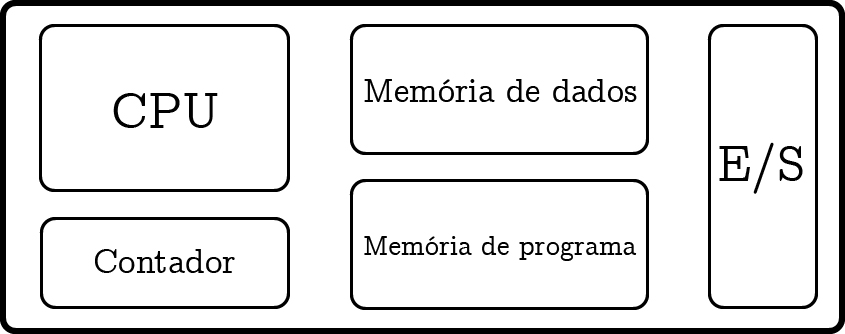
\includegraphics[scale=0.25]{Microcontrolador.jpg}
    \caption{Microcontrolador}
    \label{MCU}
\end{figure}

A \textsf{\textbf{CPU}}, ou processador, é a responsável por todo o processamento - \textit{sequencial} -  das instruções contidas na memória de programa.

A \textbf{\textsf{memória de dados}},  geralmente uma RAM, é utilizada essencialmente
para mapear os registradores, de controle e de dados.

A \textbf{\textsf{memória de programa}}, uma ROM, contém as intruções a serem lidas e executadas pela \textit{CPU}.

A \textbf{\textsf{interface de entrada e saída de periféricos}} é, de fato, a responsável pela comunicação e interação do MCU com o ambiente externo. É através dela que são conectados sensores, atuadores, displays e memórias secundárias.


Amplamente utilizado em sistemas embarcados, os \textit{MCUs} apresentam um baixo consumo energético e tamanho extremamente reduzido quando comparado com computadores pessoais (\textit{PCs}).

Os microcontroladores tiveram um grande impulso e popularidade com o advento do Arduino, que utiliza microcontroladores da \textit{ATMEL}. Outras empresas que desenvolvem microcontroladores em larga escala são a  \textit{Texas Instruments} (MSP), \textit{Microchip} (PIC) e \textit{Expressif Systems} (ESP8266).

\vspace{5pt}

           \begin{tcolorbox}[colbacktitle=blue!70!white!50,
title={\vspace{-13pt}
\includegraphics[scale=0.033]{interrogacao.png} \hspace{2pt} \textsf{\textbf{Você sabia?}\vspace{4pt}}},coltitle=black, colback=white,arc=4mm, outer arc=3.5mm]
\raggedright

O \textit{Kinetis KL03}, da \textit{Freescale}, é o atual menor microcontrolador de 32-bits do mundo com dimensões de 1.6 x 2.0 mm! 
\end{tcolorbox}

\section{Sinais Analógicos e Digitais}
O mundo eletrônico comunica entre si através de sinais elétricos dos quais podem ser descritos como \textsf{\textbf{digitais}} ou \textsf{\textbf{analógicos}}.

\subsection{Sinal Analógico}
   Sinais digitais representam \textbf{\textsf{valores contínuos}} em função do tempo. Geralmente, em circuitos digitais, os sinais analógicos expressam a saída de sensores.
   
   \begin{figure}[ht]
   \centering
   \label{Sinal-Analogico}
    \begin{tikzpicture}
      %\draw[->] (-2,0) -- (5.3,0);
      %\draw[->] (-2,-2) -- (-2,2);
      {\draw[blue,smooth,samples=100,domain= 0.7:7.455]
      plot(\x,{2.4+2*sin(\x r*4 )});}
      \begin{axis}[
        width=9.3cm,
        height=6cm,
        x axis line style={-stealth},
        y axis line style={-stealth},
       % title={Square wave},
        xticklabels={},
        ymax = 1.2,xmax=7.5,
        axis lines*=center,
        ytick={0.5,1},
        xlabel={Tempo},
        ylabel={Amplitude},
        xlabel near ticks,
        ylabel near ticks]
        \end{axis}
    \end{tikzpicture}
    \caption{Sinal Analógico}   
   \end{figure}
    
   
    
\subsection{Sinal Digital}
    Os sinais digitais representam, ao contrário dos analógicos, \textbf{\textsf{valores discretos}}. Na grande maioria dos circuitos digitais, podem assumir apenas dois valores: \textbf{\textbf{0}} e \textbf{\textbf{1}}.
   \begin{figure}[ht]
    \centering
    \label{Sinal-Digital}
    \begin{tikzpicture}
        \begin{axis}[
        width=8.3cm,
        height=6cm,
        x axis line style={-stealth},
        y axis line style={-stealth},
       % title={Square wave},
        xticklabels={},
        ymax = 1.2,xmax=7.5,
        axis lines*=center,
        ytick={0.5,1},
        xlabel={Tempo},
        ylabel={Amplitude},
        xlabel near ticks,
        ylabel near ticks]
        \addplot+[thick,mark=none,const plot]
        coordinates
        {(0,0) (0,1) (1,0) (2,1) (3,0) (4,1) (5,0) (6,1) (7,0)};
        \end{axis}
        \end{tikzpicture}
    \caption{Sinal Digital}
    \end{figure}

\subsubsection{Clock}
Gerado por um gerador de clock (geralmente um cristal oscilador), o clock é um valor que varia entre nível lógico alto e baixo - \textit{onda quadrada} em uma frequência específica e é usado na coordenação de ações de circuitos digitais.

\section{\textit{Wi-Fi}}

O protocolo de rede sem fio \textit{IEEE 802.11}, mais conhecido como \textit{Wi-Fi}, alterou o perfil de uso da \textit{Internet}, a conectando a cada vez mais dispositivos e pessoas.

Varios padrões do protocolo foram desenvolvidos, com diferentes frequências, largura de banda, velocidades de transferência e alcance. A Tabela \ref{WiFi-table} ilustra os principais protocolos \textit{Wi-Fi}:
 
\begin{table}[ht]
    \centering
    \caption{ Principais protocolos Wi-Fi\label{WiFi-table}}
    \begin{tcolorbox}[tabularx={c |Y|Y|Y|Y}]
    \textbf{Protocolo} & \textbf{Freq.}     & \textbf{Larg.}     & \textbf{\small{Alcance}}    & \textbf{\small{Alcance}} \\
    & (GHz) & de banda & \textit{indoor } (m) & \textit{outdoor } (m)\\
    & & (MHz) & & \\\hline
    \emph{802.11}   & 2.4 & 22 &  20 &  100 \\\hline
    \emph{802.11b} & 2.4 & 22 &  35 &  140 \\\hline
    \emph{802.11g}  & 2.4 & 20 &  38 &  140 \\\hline
    \emph{802.11n}   & 2.4/5 & 20/40 & 70/70 & 250/250 
    \end{tcolorbox}
\end{table}


% ------------------------------------------------------------
\chapter{O ESP8266}
% ------------------------------------------------------------

\lettrine[nindent=0.35em,lhang=0.40,loversize=0.3]{O}{ ESP8266} é um microcontrolador de 32-bits com \textit{Wi-Fi} integrado desenvolvido pela chinesa \textit{Espressif Systems} e surgido, em meados de 2014, para suprir a contínua demanda por uma plataforma de \textsf{\textbf{baixo consumo}} energético, \textsf{\textbf{tamanho reduzido}} e  \textsf{\textbf{desempenho confiável}} na industria de \textit{IoT}.

Assim como a maioria dos modelos Arduino, o ESP possui GPIOs (Pinos de entrada e saída de propósito geral) e suporte a PWM (Modulação por largura de pulso). O upload do firmware é feito também pela UART (RX/TX), porém o ESP8266 conta com upload OTA (over-the-air), que é a gravação através de uma rede.  

\newpage

\section{CPU}

O ESP8266 utiliza o processador Tensilica L106 32-bit, RISC e que possui velocidade de clock de 80MHz.

          \begin{tcolorbox}[colbacktitle=green!50!white!60,
title={\vspace{-13pt}
\includegraphics[scale=0.032]{notebook.png} \hspace{2pt} \textsf{\textbf{Na Prática...}\vspace{4pt}}},coltitle=black, colback=white,arc=4mm, outer arc=3.5mm]
\raggedright

Facilmente, podemos alterar - \textit{overclock} - da \textit{CPU} para 160MHz! Para isso, basta adicionarmos o seguinte código no escopo geral do código:
\begin{lstlisting}
extern "C" {
    bool system\_update\_cpu\_freq(int);
}

\end{lstlisting}

E na função \emph{setup()}:
\begin{lstlisting}
void setup(){
    ...
    system\_update\_cpu\_freq(160);
    ...
}
\end{lstlisting}
\end{tcolorbox}


\section{Modem \textit{Wi-Fi}}
Com um completo e autônomo sistema de conexão \textit{Wi-Fi} (suporte a \textit{802.11b/g/n/e/i}), o \textit{ESP8266} pode tanto estabelecer uma rede própria, em modo \textbf{\textsf{AP}}, ou um se conectar a um \textit{host}, em modo \textbf{\textsf{STA}}. Possui ainda o modo \textbf{\textsf{AP\_STA}}, que cria uma rede, mas também acessa uma \textit{station}, simultaneamente. 

Pode ser implementado como um "módulo \emph{WiFi}" em conjunto com qualquer microcontrolador e comunicá-los através de interfaces \textbf{\textsf{SPI}}, \textbf{\textsf{I2C}} e \textbf{\textsf{UART}} disponíveis na placa. 



\section{Alimentação}

A faixa de tensão de operação do \textit{ESP8266} é de \textbf{\textsf{2.5V}} à \textbf{\textsf{3.6V}}, sendo necessário o fornecimento de, ao menos, \textbf{\textsf{500mA}} de corrente.
\vspace{5pt}

\begin{tcolorbox}[colbacktitle=red!65!white,
title={\vspace{-13pt}
\includegraphics[scale=0.014]{x.png} \hspace{2pt} \textsf{\textbf{CUIDADO!}\vspace{2pt}}},coltitle=black, colback=white,arc=4mm, outer arc=3.5mm]
\raggedright
 O ESP8266 \textsf{\textbf{não é}} tolerante à 5V. Alimentá-lo com essa tensão pode - \textit{e vai} - danificar seu dispositivo.
\end{tcolorbox}




\section{Modos de operação}
O \textit{ESP8266} possui \textbf{\textsf{três}} modos de boot: 

\begin{table}[!ht]
\centering
\footnotesize{
\label{Modos-Energia}
\caption{Modos de boot}
\begin{tabular}{>{\bfseries}lp{5.35cm}}
\toprule
UART mode & Modo deve ser selecionado para realizar o upload de um novo \textit{firmware} no MCU. A \textbf{\textsf{GPIO0}} deve estar em \textbf{\textsf{GND} / \textbf{\textsf{GPIO2}} em \textbf{\textsf{VCC}}}. \\\midrule
Flash mode & Neste modo, o boot é realizado da memória \textit{flash}. O último firmware gravado será executado. A \textbf{\textsf{GPIO0}} deve estar em \textbf{\textsf{VCC}} / \textbf{\textsf{GPIO2}} em \textbf{\textsf{VCC}} \\\midrule
SDIO mode & Quando habilitado, o MCU realiza o boot não da memória \textit{flash}, mas sim de um cartão SD, usando protocolo \textit{SPI}. A \textbf{\textsf{GPIO15}} deve estar em \textbf{\textsf{VCC}}. \\\bottomrule
\end{tabular}
}
\end{table}

\section{GPIOS}

O \textit{ESP8266} possui 17 pinos GPIO que podem assumir varias funções através da devida programação de seus registradores. Cada um dos pinos pode ser configurado com \textbf{\textsf{pull-up}} ou \textbf{\textsf{pull-down}} interno e também alta impedância. Possui um pino \textbf{\textsf{ADC}}, TOUT $\perp$ 9, de resolução de 1024 bits, porém sua alimentação deve ser limitada de 0 a 1V.


\section{\textit{I2C}}
    \textit{I2C} (\textit{Inter-integrated Circuit}) é um protocolo de comunicação \textit{master/slave} entre dispositivos que se baseia em um barramento de apenas duas vias: \textbf{\textsf{SDA}} (Serial Data) por onde são transmitidos e recebidos os dados e \textbf{\textsf{SCL}} (Serial Clock) que dita a temporização do tráfego das informações. O grande diferencial do protocolo é que são permitidos, teoricamente, até 127 dispositivos distintos comunicando através de um mesmo barramento.
    
    O ESP8266 possui suporte a interface \textit{I2C}, tanto como Master quanto Slave, para comunicação com outros microcontroladores e outros equipamentos periféricos, como sensores. A pinagem do barramento é vista pela Tabela \ref{I2C-table} abaixo:
     
\begin{table}[ht]
    \centering
    \caption{Pinagem I2C \label{I2C-table}}
    \begin{tcolorbox}[tabularx={c |Y|Y}]
    \textbf{Pino} & \textbf{Função}     & \textbf{Descrição}    \\\hline
    \emph{GPIO02 $\perp$ 14}      & SDA   & Pino de dados   \\
    \emph{MTMS $\perp$ 9}          & SCL   & Pino de Clock           
    \end{tcolorbox}
\end{table}     
     
          
%\section{I2S}

%\begin{table}[ht]
%    \centering
%    \caption{Pinagem I2S \label{I2S-table}}
%    \begin{tcolorbox}[tabularx={c |Y|Y}]
%    \textbf{Pino} & \textbf{Função}     & \textbf{Descrição}    \\\hline
%    \emph{GPIO02 $\perp$ 14}      & SDA   & Pino de dados   \\
%    \emph{MTMS $\perp$ 9}          & SCL   & Pino de Clock           
%    \end{tcolorbox}
%\end{table}     
     

\section{UART}

O \textit{ESP8266} possui \textbf{\textsf{duas}} interfaces \textit{UART }(Universal Asynchronous Receiver/Transmitter) que podem alcançar\textbf{ \textsf{4.5 Mbps}} de velocidade de transferência: a \textbf{\textsf{UART0}}, que pode ser usada para comunicação bidirecional; e a \textbf{\textsf{UART1}} que apenas envia dados, por seu pino \textit{TX} (geralmente usado como \textit{debugger}).

\begin{table}[ht]
    \centering
    \caption{Pinagem UART \label{UART-table}}
    \begin{tcolorbox}[tabularx={c |Y|Y}]
    \textbf{Pino} & \textbf{Função}     & \textbf{Descrição}    \\\hline
    \emph{GPIO1 $\perp$ 26}      & TX0   & \small{Transmissão Serial}   \\
    \emph{GPIO3 $\perp$ 25}          & RX0   & \small{Recepção Serial}  \\
    \emph{GPIO2 $\perp$ 23}          & TX1   & \small{Transmissão Serial}          
    \end{tcolorbox}
\end{table}     
     

\section{Watchdog}
\textit{Watchdog timer} é um circuito contador independente do clock principal e que serve como um recurso de segurança adicional.

Uma das maiores diferenças entre o \textit{ESP8266} e um MCU utilizado em alguns modelos \textit{Arduino}, é o fato de que o microcontrolador da \textit{Espressif} executa varias tarefas em segundo plano: mantém a conexão do modem Wi-Fi, gerencia a pilha do protocolo TCP/IP, etc. Para manter a execução destas tarefas, ele possui dois watchdog timers: \textbf{\textsf{SW\_WDT}}, que é via software; e \textbf{\textsf{HW\_WDT}}, via Hardware. Caso uma função gere um loop longo (mais de 3 segundos) onde não haja alimentação do watchdog, o microcontrolador irá reiniciar, justamente para manter a execução das tarefas de segundo plano.

Consulte a subseção \ref{subsec:yield-oi} para melhor entendimento de como o software controla o \textit{timer} do \textit{Watchdog}. Este tópico tratará da função \emph{yield()}, que realiza a alimentação do \textbf{\textsf{SW\_WDT}}.

\section{PWM}

\textit{PWM} (ou \textit{Modulação por Largura de Pulso}) se refere a um tipo de sinal digital que permite a variação do tempo, de forma analógica, em que um sinal digital assume nível lógico alto. Desta forma, é possível modular a largura do pulso (duração do nível alto) e gerar sinais de tensões intermediárias. 
           \begin{tcolorbox}[colbacktitle=green!50!white!60,
title={\vspace{-13pt}
\includegraphics[scale=0.032]{notebook.png} \hspace{2pt} \textsf{\textbf{Na Prática...}\vspace{4pt}}},coltitle=black, colback=white,arc=4mm, outer arc=3.5mm]
\raggedright
Para usarmos um pino como saída de PWM:
\begin{lstlisting}
analogWrite(pino, valor); 
\end{lstlisting}
Alterar a frequência do sinal:
\begin{lstlisting}
analogWriteFreq(novaFrequencia); //100 Hz and 1 kHz
\end{lstlisting}
Alterar o \textit{range} do sinal:
\begin{lstlisting}
analogWriteRange(novoRange); // 1024 por padrão -> 2^10
\end{lstlisting}

\end{tcolorbox}

\vspace{7pt}
           \begin{tcolorbox}[colbacktitle=blue!70!white!50,
title={\vspace{-13pt}
\includegraphics[scale=0.033]{interrogacao.png} \hspace{2pt} \textsf{\textbf{Você sabia?}\vspace{4pt}}},coltitle=black, colback=white,arc=4mm, outer arc=3.5mm]
\raggedright

Uma clássica experiência do modelo pode ser realizada ao chavear, rapidamente, o interruptor da iluminação do seu quarto, por exemplo. A sensação será a de uma iluminação intermediária entre lâmpada desligada e normalmente acesa.

\end{tcolorbox}



O ESP8266 possui 4 pinos de interface \textit{PWM}, mas podem ser estendidos pelo usuário. A definição padrão dos pinos é dada pela Tabela \ref{PWM-table} abaixo.



\begin{table}[ht]
    \centering
    \caption{Pinagem PWM \label{PWM-table}}
    \resizebox{0.5\textheight}{!}{
    \begin{threeparttable}
        
        \begin{tcolorbox}[tabularx={X|Y}]
        \textbf{Pino} & \textbf{Função}   \\\hline
        \emph{MTDI $\perp$ 10}      & PWM0   \\
        \emph{MTDO $\perp$ 13}          & PWM1  \\
        \emph{MTMS $\perp$ 9}          & PWM2  \\
        \emph{GPIO4 $\perp$ 16}          & PWM4  \\[1ex]
        \end{tcolorbox}
    \end{threeparttable}
    }
\end{table}     
     

               
\section{Interrupção externa}
        Interrupções são eventos ou condições que levam o microcontrolador a pausar a execução de uma tarefa em andamento, executar outra temporariamente e, então, retornar para a tarefa inicial.
    
        Com exceção do pino \emph{GPIO16 $\perp$ 8}, todas as demais GPIOs do ESP8266 possuem funcionalidade de interrupção externa.
        
        \vspace{10pt}
        
           \begin{tcolorbox}[colbacktitle=green!50!white!60,
title={\vspace{-13pt}
\includegraphics[scale=0.032]{notebook.png} \hspace{2pt} \textsf{\textbf{Na Prática...}\vspace{4pt}}},coltitle=black, colback=white,arc=4mm, outer arc=3.5mm]
\raggedright
    Podemos utilizar uma interrupção que será deflagrada ao estado do sinal do pino apresentar uma curva de subida - \textit{rising} - e chamará a função \emph{resolveInterrupcao()} da seguinte forma:
    
       \begin{lstlisting} 
void setup() {
    ...
    pinMode(pinoDeInterrupcao, INPUT);
    attachInterrupt(pinoDeInterrupcao, resolveInterrupcao, "RISING");
    // Alem de "RISING", pode assumir "CHANGE" ou "FALLING"
    ...
}
    
void resolveInterrupcao() {
    ...
}
    
        
\end{lstlisting}

\end{tcolorbox}


\section{Consumo de Energia}
O ESP8266 já possui modos de consumo definidos, que gerenciam o funcionamento de algumas funcionalidades visando economia energética de acordo com cada tipo de aplicação. 

A Tabela \ref{Modos-Energia} apresenta estes modos, suas funções ativas e consumo médio.

\vspace{10pt}

\begin{table}[!ht]
\centering
\footnotesize{
\label{Modos-Energia}
\caption{Modos de Consumo Energético}
\begin{tabular}{>{\bfseries}lp{5.35cm}}
\toprule
modem-sleep & Modo usado em aplicações que requerem a CPU funcionando, como em aplicações com PWM e I2S. "Desliga" o circuito do Modem Wi-Fi enquanto mantiver uma conexão Wi-Fi sem transmissão de dados. \emph{Consumo médio: 15mA}. \\\midrule
light-sleep & Durante o modo, a CPU pode ser suspendida em aplicações como uma interruptor Wi-Fi. Sem haver transmissão de dados, a o circuito do Modem Wi-Fi pode ser desligado e a CPU suspendida para economia de consumo de energia. \emph{Consumo médio: 0.9mA.} \\\midrule
deep-light & Durante o modo, o modem Wi-Fi é totalmente desligado. Para aplicações onde existam longos intervalos de tempo sem transmissão de dados. Por exemplo, o monitoramento da temperatura ambiente, lendo dados durante um período, dormindo por outro período e acordando para reconectar a um ponto de acesso. \emph{Consumo médio: 20$\mu$A}. \\\bottomrule
\end{tabular}
}
\end{table}

\chapter{\textit{Firmware}}

\lettrine[nindent=0.35em,lhang=0.40,loversize=0.3]{O}{ firmware} traz, por padrão, o conjunto de instruções AT (PDF), porém é possível realizar o upload de outros firmwares para programação em linguagens mais comuns como o \textit{nodeMCU} (LUA) e o \textit{micropython} (Python). Ambos os firmwares baseam em um sistema interno de arquivos, com um arquivo "main" executado no boot e também possuem sua própria biblioteca que é atualizada por suas comunidades. 
Entretanto, a Arduino IDE possui, atualmente, suporte ao ESP8266, tornando possível a programação em Arduino (C++), utilizando, inclusive, algumas bibliotecas do mesmo sem realizar quaisquer alterações.

\newpage

\section{Conversores \textit{USB} para \textit{UART}}
        O ESP8266 não possui, nativamente, interface para comunicação USB, porém existem conversores que facilitam a comunicação entre o microcontrolador e um PC para realização do upload do programa, por exemplo. 

É possível ainda utilizar de dispositivos que já possuam um conversor interno para realizar o upload, como o Arduino UNO. Interligando os pinos de UART dos dois dispositivos (TX(ESP) $\rightarrow$ RX(Arduino) e RX(ESP) $\rightarrow$ TX(Arduino)) é possível realizar a comunicação do \textit{ESP8266} com um PC através do conversor USB do Arduino.

\vspace{10pt}

\begin{tcolorbox}[colbacktitle=yellow!60!white,
title={\vspace{-13pt}
\includegraphics[scale=0.03]{exclamacao.png} \hspace{2pt} \textsf{\textbf{ATENÇÃO!}\vspace{2pt}}},coltitle=black, colback=white,arc=4mm, outer arc=3.5mm]
\raggedright
 A faixa de tensão de operação do ESP8266 é de \textsf{2.5} a \textsf{3.6V}, sendo necessário, então, um divisor de tensão do \textit{TX} (Arduino), que possui \textsf{5V}, para o \textit{RX} (ESP8266).
\end{tcolorbox}

\section{\textit{IDE Arduino}}

Implementada em \textit{Java}, a \textit{IDE Arduino} possui uma interface \textbf{\textsf{simples}} e \textbf{\textsf{objetiva}}.

Apesar de não apresentar algumas funções e macros presentes em outros editores de texto, como \textit{auto-complete} e snippets, a \textit{IDE} possui recursos interessantes ao usúario. como o \textbf{\textsf{Monitor Serial}}.

A figura \ref{IDE} exibe um \textit{screenshot} do layout do programa.
\\


\subsection{Monitor Serial}
    
    É uma interface de interação com o usuário e depuração do código compilado fornecida pela \textit{\textsf{IDE Arduino}}, onde é possível visualizar dados enviados, via comunicação serial, do MCU para um PC. É possível usá-lo, também, para envio de dados em tempo real do computador para o microcontrolador. Todos os projetos exemplificados neste livro utilizam o \textsf{\textbf{Monitor Serial}} para identificarmos as etapas de execução do programa no \textit{ESP8266}.
    
    \vspace{5pt}
    
    \begin{tcolorbox}[colbacktitle=green!50!white!60,
title={\vspace{-13pt}
\includegraphics[scale=0.032]{notebook.png} \hspace{2pt} \textsf{\textbf{Na Prática...}\vspace{4pt}}},coltitle=black, colback=white,arc=4mm, outer arc=3.5mm]
\raggedright
    
    Antes de utilizarmos o \textbf{\textsf{Monitor Serial}}, devemos nos certificar de ter inicializado a comunicação serial com seu \textit{baudrate} (tava de transferência de dados), via software:
    
    \begin{lstlisting}
void setup(){
        ...
    Serial.begin(115200);
        ...
}
    \end{lstlisting}
    
    Para escrevermos alguma mensagem no monitor, usamos a função \emph{print()}:
    
    \begin{lstlisting}
Serial.print("MENSAGEM PARA MONITOR");
    \end{lstlisting}
    
\end{tcolorbox}

%\subsection{Plotter}


\section{A Linguagem \textit{Arduino}}
\label{sec:arduino}
Baseada em \textbf{\textsf{C++}}, a linguagem de domínio específico \textit{Arduino} traz facilidades ao programador de microcontroladores com funções de leitura, escrita e depuração de pinos de I/O implementadas. Além das funções estruturais \emph{loop()} e \emph{setup()}, que guiam o desenvolvimento do software.

A DSL Arduino possui suporte à orientação a abjetos, alocação dinâmica e manipulação de ponteiros, bem como os tipos de dados aceitos por sua linguagem "mãe".

\begin{figure}[b]
    \centering
    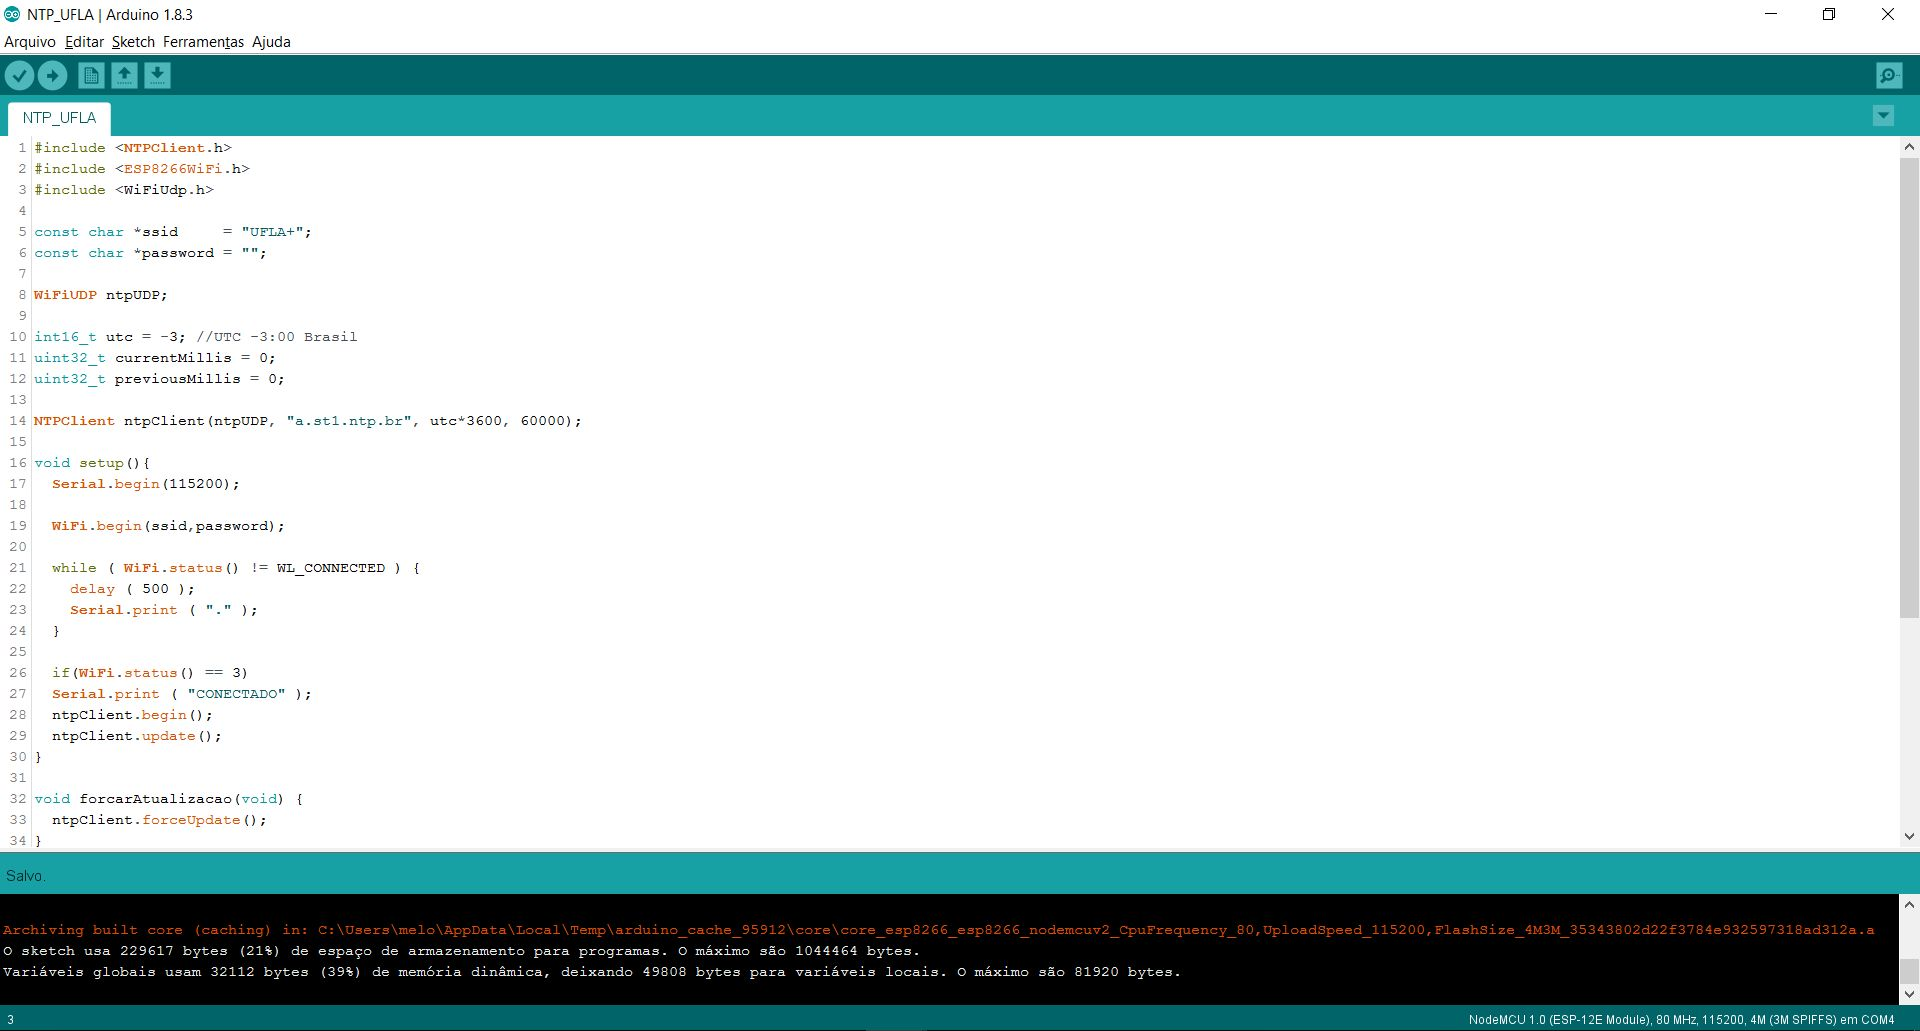
\includegraphics[scale=0.2]{Arduino.jpg}
    \caption{IDE Arduino}
    \label{IDE}
\end{figure}


\subsection{Funções Estruturais}
    Um código em Arduino possui duas funções essenciais: a \textit{loop()} e a setup():
    
    \begin{table}[!ht]
\centering
\label{Funcoes-basicas}
\caption{Funções básicas}
\footnotesize{
\begin{tabular}{>{\bfseries}lp{5.35cm}}
\toprule

void setup() & Função executada apenas uma vez após o MCU dar o boot ou reset. Nela são inicializadas variáveis e indicadas classes, setados modos de entrada ou saída dos pinos, etc. \\\midrule
void loop() & Função chamada após executar a void \textit{setup()}, que rege a execução do código, repetindo infinitas vezes seu conteúdo. Ao final de um ciclo de execução da função, é chamada a função \textit{yield()} para dar feed ao \emph{SW WDT}. \\\bottomrule
\end{tabular}
}
\end{table}
    
       \begin{lstlisting} 
void setup() {
    ...
}
    
void loop() {
    ...
}
    
        
\end{lstlisting}

    
\subsection{Timer: \textit{delay()} {\normalsize{\emph{VS}}} \textit{millis()}}
    A linguagem possui duas funções principais para contagem de tempo durante execução do programa:
    
    \begin{table}[!ht]
            \centering
            \label{timers}
            \footnotesize{
            \caption{Funções de contagem de tempo}
            \begin{tabular}{>{\bfseries}lp{5.35cm}}
            \toprule
            delay(\emph{tempo}) & Função que recebe em \emph{tempo} um valor, em millisegundos, em que o MCU irá pausar a maioria das tasks e retornar a execução normal após este período. A função, porém não desabilita interrupções e mantém os valores da porta serial (recebidos em \emph{RX}), PWM e estados dos pinos.
            
            \textit{A função delay() chama, internamente, a função} \textbf{\textsf{yield()}}.   \\\midrule
            
            millis() & Função retorna o tempo, em milisegundos, desde o início do programa atual. O valor retornado tem tipo \emph{unsigned long} e sofrerá overflow em cerca de 50 dias de execução contínua do MCU.
            
            \textit{A função millis() \textbf{\textsf{não}} chama, internamente, a função} \textbf{\textsf{yield()}}.\\\bottomrule
            \end{tabular}
            }
    \end{table}
    

\subsection{Função \textit{yield()}}
\label{subsec:yield-oi}
Uma das situações mais comuns aos novos usuários do ESP8266, é o reset inesperado -  \textit{e misterioso} - do MCU. Como visto anteriormente, o 8266 possui 2 circuitos de \textit{Watchdog} sendo um via software (SW\_WDT) e outro via Hardware (HW\_WDT). O SW\_ WDT é alimentado justamente pela função \textit{yield()}, que faz a contagem de seu timer (cerca de 3 segundos) reiniciar.

\begin{tcolorbox}[colbacktitle=green!50!white!60,
title={\vspace{-13pt}
\includegraphics[scale=0.032]{notebook.png} \hspace{2pt} \textsf{\textbf{Na Prática...}\vspace{4pt}}},coltitle=black, colback=white,arc=4mm, outer arc=3.5mm]
\raggedright
No trecho de código abaixo podemos analisar o uso do \emph{yield()} para evitar o reset do microcontrolador:
       \begin{lstlisting} 
void loop() {
    ...
    piscaLed(led,10000); // recebe o tempo em milissegundos
    ...
}
    
int piscaLed(int led,int tempo) {
    int tempoInicial = millis();
    int contador = tempoInicial;
    while (contador - tempoInicial < tempo) {
        digitalWrite(led, HIGH);
        delayMicroseconds(500000);
        digitalWrite(led, LOW);
        delayMicroseconds(500000);
        contador = millis();
        yield();
    }
}
    
    
\end{lstlisting}

Como a função \emph{piscaLed()} possui um loop interno que dura, no caso, 10 segundos, caso comentássemos a chamada da \emph{yield()}, o \emph{SW\_WDT} não seria alimentado e, em cerca de 3 segundos, o microcontrolador se reiniciaria. Podemos, analogamente, utilizar as seguintes funções que chamam internamente a \emph{yield()} para evitar o \textit{reset}:

\begin{lstlisting}
 delay();
 \end{lstlisting}
 ou
 \begin{lstlisting}
 ESP.wdtFeed(); // Esta, porem, alimenta tambem o HW_WDT
 \end{lstlisting}

\end{tcolorbox}

\begin{tcolorbox}[colbacktitle=yellow!60!white,
title={\vspace{-13pt}
\includegraphics[scale=0.03]{exclamacao.png} \hspace{2pt} \textsf{\textbf{ATENÇÃO!}\vspace{2pt}}},coltitle=black, colback=white,arc=4mm, outer arc=3.5mm]
\raggedright
 As funções \emph{delayMicroseconds()} e \emph{millis()} \textsf{\textbf{não}} chamam, internamente, a função \emph{yield().}
\end{tcolorbox}

\section{SPIFFS}
Um dos problemas enfrentados pelos programadores de microcontroladores é a limitação física da memória, de forma mais crítica, na RAM. Pensando nisso, o \textit{ESP8266} traz, nativamente, um sistema interno de arquivos baseado em um sistema \textit{SPI NOR Flash}. Não suporta criação e manipulação de diretórios, porém é possível nomear um arquivo utilizando "/", tornando possível, ao menos, fantasiara um diretório.

\vspace{8pt}

\begin{tcolorbox}[colbacktitle=green!50!white!60,
title={\vspace{-13pt}
\includegraphics[scale=0.032]{notebook.png} \hspace{2pt} \textsf{\textbf{Na Prática...}\vspace{4pt}}},coltitle=black, colback=white,arc=4mm, outer arc=3.5mm]
\raggedright

Inicia o SPIFFS
\begin{lstlisting}
SPIFFS.begin();
\end{lstlisting}

Abre um arquivo
\begin{lstlisting}
SPIFFS.open(path, mode); // mode recebe "r", "w", "a", "r+", "w+" ou "a+".
\end{lstlisting}

Remove um arquivo
\begin{lstlisting}
SPIFFS.remove(path)
\end{lstlisting}

Fecha um arquivo
\begin{lstlisting}
file.close()
\end{lstlisting}


\end{tcolorbox}

\section{PROGMEM}
Ainda pesando na limitação de hardware da memória, o ESP importa da biblioteca do Arduino uma função que possibilita a alocação de strings e variáveis na memória flash (que é bem maior) ao invés da RAM: a \textbf{\textsf{PROGMEM}}.

\vspace{10pt}

\begin{tcolorbox}[colbacktitle=green!50!white!60,
title={\vspace{-13pt}
\includegraphics[scale=0.032]{notebook.png} \hspace{2pt} \textsf{\textbf{Na Prática...}\vspace{4pt}}},coltitle=black, colback=white,arc=4mm, outer arc=3.5mm]
\raggedright
 Existem duas formas de declarar uma variável para ser armazenada em \textbf{\textsf{flash}}:
 
 \begin{lstlisting}
 const tipoDado nomeVariavel[] PROGMEM = {};
 \end{lstlisting}
 ou
 \begin{lstlisting}
 const PROGMEM tipoDado nomeVariavel[] = {}; 
 \end{lstlisting}
 
 Em ambas, após a alocação na memória, para acessar o seu conteúdo são necessários funções especiais de leitura. Por exemplo, para recuperar o valor da variável \emph{mensagem} declarada como:
 
 \begin{lstlisting}
 const char mensagem[] PROGMEM = {"ESTE LIVRO EH UMA INTRODUCAO AO IOT"}; 
 \end{lstlisting}
 
 devemos fazê-la da seguinte forma:
 
 \begin{lstlisting}
 char mensagemAux;
 for (k = 0; k < strlen_P(mensagem); k++)
  {
    mensagemAux =  pgm_read_byte_near(mensagem + k);
    Serial.print(mensagemAux);
  }
 \end{lstlisting}
\end{tcolorbox}
    
    Ao utilizar o \textbf{\textsf{Monitor Serial}} como debugger ou uma interface de numerosas mensagens, estamos propícios a, facilmente, consumir muita memória RAM durante as chamadas funções de impressão como:
    \begin{lstlisting}
    Serial.print("ESTE LIVRO EH UMA INTRODUCAO AO IOT"); 
    \end{lstlisting}
    Nestas chamadas, todas os dados são armazenados, por padrão, na RAM do dispositivo. Para contornar isso, podemos modificá-las adicionando a macro \emph{F()}, que altera este armazenamento para a flash:
    \begin{lstlisting}
    Serial.print(F("ESTE LIVRO EH UMA INTRODUCAO AO IOT")); 
    \end{lstlisting}
    
    
\begin{tcolorbox}[colbacktitle=yellow!60!white,
title={\vspace{-13pt}
\includegraphics[scale=0.03]{exclamacao.png} \hspace{2pt} \textsf{\textbf{ATENÇÃO!}\vspace{2pt}}},coltitle=black, colback=white,arc=4mm, outer arc=3.5mm]
\raggedright
 Todas as variáveis devem ser definidas globalmente ou definidas como estáticas, \textbf{\textsf{caso contrário}} o \textsf{\textbf{PROGMEM}} não funcionará.
\end{tcolorbox}
    






%\section{Primeiro programa}



% ------------------------------------------------------------
%\chapter{ESP8266 {\normalsize{\emph{VS}}} Arduino}
% ------------------------------------------------------------




% ------------------------------------------------------------
\chapter{Exemplos e Aplicações}
% ------------------------------------------------------------
\lettrine[nindent=0.35em,lhang=0.40,loversize=0.3]{T}{odas} implementações do capítulo utilizam a linguagem \textit{Arduino} e a \textit{IDE Arduino} como framework para desenvolvimento no ESP8266. Foram selecionados exemplos básicos, como o clássico \textbf{\textsf{Blink}}; que utilizem o acesso à Internet para obtenção de dados, como o relógio usando \textbf{\textsf{NTP}}; de comunicação entre dispositivos sem fio através de protocolos\textbf{ \textsf{TCP}} e \textbf{\textsf{MQTT}}; leitura e processamento de dados de \textbf{\textsf{Sensores}}; um \textbf{\textsf{Web Server}} e, por fim, exemplos de construção de um \textbf{\textsf{Datalogger}} usando uma nuvem ou a própria memória flash do dispositivo.

\newpage

\section{\textit{Blink}}
\begin{lstlisting} 

#define LED 5

void setup() {
    pinMode(LED, OUTPUT);
}

void loop() {
    digitalWrite(LED,HIGH);
    delay(1000);
    digitalWrite(LED,LOW);
    delay(1000);
}


\end{lstlisting}

\newpage

\section{Relógio - \textit{NTP}}

       \begin{lstlisting} 

#include <NTPClient.h>
#include <ESP8266WiFi.h>
#include <WiFiUdp.h>

/*
CONFIGURACAO WIFI
*/
const char *ssid     = "ssid_rede";
const char *password = "senha_rede";

WiFiUDP ntpUDP;

//UTC -3:00 Brasil
int16_t utc = -3; 
uint32_t atualMillis = 0;
uint32_t anteriorMillis = 0;

NTPClient timeClient(ntpUDP, "a.st1.ntp.br", utc*3600, 60000);

void setup(){
  Serial.begin(115200);
  
  WiFi.begin(ssid, password);

  while ( WiFi.status() != WL_CONNECTED ) {
    delay ( 500 );
    Serial.print ( "." );
  }

  timeClient.begin();
  timeClient.update();
}

void forcaUpdate(void) {
  timeClient.forceUpdate();
}

void checkOST(void) {
  atualMillis = millis();//Tempo atual em ms
  //Logica de verificacao do tempo
  if (atualMillis - anteriorMillis > 1000) {
    anteriorMillis = atualMillis;    // Salva o tempo atual
    Serial.println(timeClient.getFormattedTime());
  }
}

void loop() {
  //Chama a verificacao de tempo
  checkOST();
}

\end{lstlisting}

\newpage

\section{Comunicação entre \textit{ESP8266} e \textit{Arduino} via \textit{I2C}}

\subsection{\textit{Master} - \textit{ESP8266}}

\begin{lstlisting}
#include <Wire.h>
 
 
void setup() {
  Wire.begin();
  Serial.begin(115200);
  pinMode(LED_BUILTIN, OUTPUT);
}
 
void loop() {
  Wire.beginTransmission(2);
  Wire.write("Oi, Arduino");
  Wire.endTransmission();
 
  int data_available = Wire.requestFrom(2, 1);
  if(data_available) {
    String slaveResp = Wire.read();
    if(slaveResp=="Oi, ESP"){
      digitalWrite(LED_BUILTIN, HIGH);
      Wire.write(led_status);
    } else{
      digitalWrite(LED_BUILTIN, LOW);
    }
    Serial.println(slaveResp);
  } 
  delay(100);
}

\end{lstlisting}

\newpage

\subsection{\textit{Slave} - \textit{Arduino}}

\begin{lstlisting}


#include <Wire.h>
 

String rec\_value = "";
 
void setup() {
  Wire.begin(2);
  Wire.onReceive(receiveCallback);
  Wire.onRequest(requestCallback);
  pinMode(LED_BUILTIN, OUTPUT);
  Serial.begin(115200);
}
 
 
void loop() {
}
 
void receiveCallback(int bytes)
{
  if(Wire.available() != 0)
  {
    for(int i = 0; i< bytes; i++)
    {
      rec_value = Wire.read();
      Serial.print("Recebido: ");
      Serial.println(rec_value);
    }
    if(rec_value=="Oi, Arduino"){
      digitalWrite(LED_BUILTIN, LOW);
    } else {
      digitalWrite(LED_BUILTIN, HIGH);
    }
  }
}
 
void requestCallback(int bytes) {
  Wire.write("Oi, Esp");
}

\end{lstlisting}
\newpage

\section{Controle remoto de aparelhos via \textit{MQTT}}

\begin{lstlisting}

#include <IRremoteESP8266.h>
#include <IRsend.h>
#include <ESP8266WiFi.h>
#include <PubSubClient.h>

// Valores lidos pelo controle remoto
#define SamsungPower        0xE0E040BF
#define SamsungSource        0xE0E0807F
#define SamsungExit        0xE0E0B44B
#define SamsungUp        0xE0E006F9
#define SamsungDown        0xE0E08679
#define SamsungRight        0xE0E046B9
#define SamsungLeft        0xE0E0A659
#define SamsungSelect        0xE0E016E9
#define SamsungUpVol        0xE0E0E01F
#define SamsungDownVol        0xE0E0D02F
#define SamsungUpCh        0xE0E048B7
#define SamsungDownCh        0xE0E008F7
#define SamsungMute        0xE0E0F00F

// Inicia o pino 12 para saida de IR
IRsend irsend(12);
 
/*
 CONFIGURACAO WIFI
*/ 
const char* ssid = "ssid_rede"; 
const char* password =  "senha_rede"; 
// Endereco do servidor mqtt
const char* mqttServer = "m13.cloudmqtt.com"; 
// Porta do Broker
const int mqttPort = 11111;
// Nome de usuario fornecido pelo broker
const char* mqttUser = "userMqtt";
const char* mqttPassword = "passMqtt"; 
WiFiClient espClient;
PubSubClient client(espClient);

unsigned long initTime;
unsigned long posTime;

void mqtt_callback(char* topic, byte* payload, unsigned int length);

void setup() {
  irsend.begin();
  WiFi.begin(ssid, password);
 
  while (WiFi.status() != WL_CONNECTED) {
    delay(500);
  }
 
  client.setServer(mqttServer, mqttPort);
  client.setCallback(callback);

  // publica("tópico", "mensagem")
  client.publish("/node03","conecao_estabelecida");
  // Inscreve em um topico
  client.subscribe("/node03/tv");
 
}
 
void callback(char* topic, byte* payload, unsigned int length) {
    
    String mensagem;
    //obtem a string do payload recebido
    for(int i = 0; i < length; i++) 
    {
       char c = (char)payload[i];
       mensagem += c;
    }
  
    if (mensagem.equals("power"))
    {
      initTime = millis();
      posTime = initTime;
      while(posTime<= initTime+50){
       irsend.sendSAMSUNG(SamsungPower, SAMSUNG_BITS, 0);  // hex value, 16 bits, no repeat
       irsend.sendSAMSUNG(SamsungPower, SAMSUNG_BITS, 1);  // hex value, 16 bits, repeat
       posTime = millis();
      }
    }
    
    else if (mensagem.equals("source"))
    {
      initTime = millis();
      posTime = initTime;
      while(posTime<= initTime+50){
       irsend.sendSAMSUNG(SamsungSource, SAMSUNG_BITS, 0);  // hex value, 16 bits, no repeat
       irsend.sendSAMSUNG(SamsungSource, SAMSUNG_BITS, 1);  // hex value, 16 bits, repeat
       posTime = millis();
      }
    }
    
    else if (mensagem.equals("select"))
    {
       irsend.sendSAMSUNG(SamsungSelect, SAMSUNG_BITS, 0);  // hex value, 16 bits, no repeat
    }

  else if (mensagem.equals("exit"))
    {
       irsend.sendSAMSUNG(SamsungExit, SAMSUNG_BITS, 0);  // hex value, 16 bits, no repeat
    }
    
    else if (mensagem.equals("up"))
    {
       irsend.sendSAMSUNG(SamsungUp, SAMSUNG_BITS, 0);  // hex value, 16 bits, no repeat
    }

    else if (mensagem.equals("down"))
    {
       irsend.sendSAMSUNG(SamsungDown, SAMSUNG_BITS, 0);  // hex value, 16 bits, no repeat
    }

    else if (mensagem.equals("right"))
    {
      irsend.sendSAMSUNG(SamsungRight, SAMSUNG_BITS, 0);  // hex value, 16 bits, no repeat
    }

    else if (mensagem.equals("left"))
    {
      irsend.sendSAMSUNG(SamsungLeft, SAMSUNG_BITS, 0);  // hex value, 16 bits, no repeat
    }
    
    else if (mensagem.equals("volup"))
    {
      irsend.sendSAMSUNG(SamsungUpVol, SAMSUNG_BITS, 0);  // hex value, 16 bits, no repeat     
    }

    else if (mensagem.equals("voldown"))
    {
       irsend.sendSAMSUNG(SamsungDownVol, SAMSUNG_BITS, 0);  // hex value, 16 bits, no repeat
    }

    else if (mensagem.equals("chup"))
    {
       irsend.sendSAMSUNG(SamsungUpCh, SAMSUNG_BITS, 0);  // hex value, 16 bits, no repeat
    }

    else if (mensagem.equals("chdown"))
    {
       irsend.sendSAMSUNG(SamsungDownCh, SAMSUNG_BITS, 0);  // hex value, 16 bits, no repeat
    }
    
    else if (mensagem.equals("mute"))
    {
       irsend.sendSAMSUNG(SamsungMute, SAMSUNG_BITS, 0);  // hex value, 16 bits, no repeat
    }
}
 
void loop() {
  client.loop();
}

\end{lstlisting}
\newpage

\section{\textit{Web Server} para envio de mensagens para um \textit{channel} do \textit{Slack}}
\begin{lstlisting} 

    #include <ESP8266WiFi.h>
    
    /*
     CONFIGURACAO WIFI
     */
    const char* ssid = "ssid_rede";
    const char* password = "senha_rede";
    WiFiServer server(80);
    
    /*
     CONFIGURACAO SLACK
     */
    // url do webhooks gerado no slack
    const String slack_hook_url = "https://hooks.slack.com/services/*****/******/******";
    // url do icone usado pelo usuario criado pelo hooks
    const String slack_icon_url = "https://pbs.twimg.com/profile_images/1462227900/cda288d94c3e99d0ccc4e8d1c61d7073_normal.jpg";
    const String slack_message = "#GoEMakers - mensagem enviada pelo ESP8266 by Arduino Firmware";
    const String slack_username = "meu_esp";
    
    void setup()
    { 
      Serial.begin(115200);
    
      WiFi.begin(ssid, password);
    
      Serial.print("Conectando a ");
      Serial.print(ssid);
      while (WiFi.status() != WL_CONNECTED)
      {
        delay(500);
        Serial.print(".");
      }
      Serial.println();
    
      Serial.println("Connectado!");
      Serial.print("Endereco IP: ");
      Serial.println(WiFi.localIP());
    
      server.begin();
    }
    
    void consultaServidor(){
      WiFiClient client = server.available();
      if (!client) {
        return;
      }
      String leitura = client.readStringUntil('\r');
      Serial.println(leitura);
      client.flush();
    
      String buf = "";
      
      buf += "HTTP/1.1 200 OK\r\nContent-Type: text/html\r\n\r\n<!DOCTYPE HTML>\r\n";
      buf += "<html lang=\"en\"><head><meta charset=\"UTF-8\" name=\"viewport\" content=\"width=device-width, initial-scale=1, user-scalable=no\"/>\r\n";
      buf += "<title>EMakers - Curso ESP8266</title>";
      buf += "<style>.c{text-align: center;} .titulo{color: white;} div,input{padding:5px;font-size:1em;background-color:#1fa3ec;} input{width:30\%;} body{text-align: center;font-family:verdana;} button{border:0;border-radius:0.3rem;background-color:#1fa3ec;color:#fff;line-height:2.4rem;font-size:1.2rem;width:20\%;} </style>";
      buf += "</head>";
      buf += "<script> function mudaCor(el){el.style.backgroundColor = '#000000';}</script>";
      buf += "<div><h1 class=\"titulo\">EMakers - Curso ESP8266</h1></div>";
      buf += "<h3>Botão de envio de mensagens Slack</h3>";
      buf += "<p>Mensagem_1: <a href=\"?function=mensagem1\"><button onclick=\"mudaCor(this)\">ENVIAR</button></a></p>";
      buf += "<p>Mensagem_2: <a href=\"?function=mensagem2\"><button onclick=\"mudaCor(this)\">ENVIAR</button></a></p>";
      buf += "<div class=\"titulo\"> <p>Desenvolvido por Gabriel Melo</p>";
      buf += "</html>\n";
    
      client.print(buf);
      client.flush();
    
      if (leitura.indexOf("mensagem1") != -1){
        mensagemParaSlack("oi, slack");
        Serial.println("Mensagem Enviada!");
      }
      else if (leitura.indexOf("mensagem2") != -1){
        mensagemParaSlack("tchau, slack");
        Serial.println("Mensagem Enviada!");
      }
      else {
        Serial.println("Requisicao invalida");
        client.stop();
      }
    }
    
    bool mensagemParaSlack(String msg)
    {
      const char* host = "hooks.slack.com";
      Serial.print("Conectando a  ");
      Serial.println(host);
    
      // Criar conexao TCP
      WiFiClientSecure client;
      const int httpsPort = 443;
      if (!client.connect(host, httpsPort)) {
        Serial.println("Falha na conexao :-(");
        return false;
      }
    
      //Criacao da URI para requisicao
    
      Serial.print("Postando em: ");
      Serial.println(slack_hook_url);
    
      String postData="payload={\"link_names\": 1, \"icon_url\": \"" + slack_icon_url + "\", \"username\": \"" + slack_username + "\", \"text\": \"" + msg + "\"}";
    
      //Envio da requisicao para o servidor
      client.print(String("POST ") + slack_hook_url + " HTTP/1.1\r\n" +
                   "Host: " + host + "\r\n" +
                   "Content-Type: application/x-www-form-urlencoded\r\n" +
                   "Connection: close" + "\r\n" +
                   "Content-Length:" + postData.length() + "\r\n" +
                   "\r\n" + postData);
      Serial.println("Requisicao enviada");
      String line = client.readStringUntil('\n');
      Serial.printf("Resposta: ");
      Serial.println(line);
      if (line.startsWith("HTTP/1.1 200 OK")) {
        return true;
      } else {
        return false;
      }
    }
    
    void loop(){
      consultaServidor();
    }

\end{lstlisting}

\newpage

\section{Controle de ponto usando RFID}

\begin{lstlisting}

    #include <ESP8266WiFi.h>
    #include <MFRC522.h>
    #include <SPI.h>
    
    #define SS_PIN 4
    #define RST_PIN 5
    MFRC522 mfrc522(SS_PIN, RST_PIN);
    
    String msg = "";
    char st[20];
    
    /*
    CONFIGURACAO WIFI
    */
    const char *ssid     = "ssid_rede";
    const char *password = "senha_rede";
    
    /*
     CONFIGURACAO SLACK
     */
    // url do webhooks gerado no slack
    const String slack_hook_url = "https://hooks.slack.com/services/*****/******/******";
    // url do icone usado pelo usuario criado pelo hooks
    const String slack_icon_url = "https://pbs.twimg.com/profile_images/1462227900/cda288d94c3e99d0ccc4e8d1c61d7073_normal.jpg";
    const String slack_message = "#GoEMakers - mensagem enviada pelo ESP8266 by Arduino Firmware";
    const String slack_username = "meu_esp";
    
    void setup() 
    {
      Serial.begin(9600); // Inicia a serial
      Serial.println();
        WiFi.begin(ssid, password);
    
      Serial.print("Connecting");
      while (WiFi.status() != WL_CONNECTED)
      {
        delay(500);
        Serial.print(".");
      }
      Serial.println();
    
      Serial.print("Connected, IP address: ");
      Serial.println(WiFi.localIP());
    
      SPI.begin();    // Inicia  SPI bus
      mfrc522.PCD_Init(); // Inicia MFRC522
      Serial.println("Aproxime o seu cartao do leitor...");
    
    }
    
    
    bool mensagemParaSlack(String msg) {
      const char* host = "hooks.slack.com";
      Serial.print("Conectando a  ");
      Serial.println(host);
    
      // Criar conexao TCP
      WiFiClientSecure client;
      const int httpsPort = 443;
      if (!client.connect(host, httpsPort)) {
        Serial.println("Falha na conexao :-(");
        return false;
      }
    
      //Criacao da URI para requisicao
    
      Serial.print("Postando em: ");
      Serial.println(slack_hook_url);
    
      String postData="payload={\"link_names\": 1, \"icon_url\": \"" + slack_icon_url + "\", \"username\": \"" + slack_username + "\", \"text\": \"" + msg + "\"}";
    
      //Envio da requisicao para o servidor
      client.print(String("POST ") + slack_hook_url + " HTTP/1.1\r\n" +
                   "Host: " + host + "\r\n" +
                   "Content-Type: application/x-www-form-urlencoded\r\n" +
                   "Connection: close" + "\r\n" +
                   "Content-Length:" + postData.length() + "\r\n" +
                   "\r\n" + postData);
      Serial.println("Requisicao enviada");
      String line = client.readStringUntil('\n');
      Serial.printf("Resposta: ");
      Serial.println(line);
      if (line.startsWith("HTTP/1.1 200 OK")) {
        return true;
      } else {
        return false;
      }
    }
    
    void loop() 
    {
      //Procura novos cards
      if ( ! mfrc522.PICC_IsNewCardPresent()) 
      {
        return;
      }
      //Seleciona um card
      if ( ! mfrc522.PICC_ReadCardSerial()) 
      {
        return;
      }
      //Mostra UID na serial
      Serial.print("UID da tag :");
      String conteudo= "";
      byte letra;
      for (byte i = 0; i < mfrc522.uid.size; i++) 
      {
         Serial.print(mfrc522.uid.uidByte[i] < 0x10 ? " 0" : " ");
         Serial.print(mfrc522.uid.uidByte[i], HEX);
         conteudo.concat(String(mfrc522.uid.uidByte[i] < 0x10 ? " 0" : " "));
         conteudo.concat(String(mfrc522.uid.uidByte[i], HEX));
      }
      Serial.println();
      Serial.print("Mensagem : ");
      conteudo.toUpperCase();
    
      if (conteudo.substring(1) == "64 96 35 24") //UID 2 - Cartao
      {
        msg = "Gabriel Marques de Melo - Chegou na sala!";
        mensagemParaSlack(msg);
        Serial.println(msg);
        Serial.println();
        delay(2000);
      }
    } 

\end{lstlisting}

\newpage

\section{Monitor de temperatura ambiente com \textit{DHT11}}

\begin{lstlisting}

    #include "DHT.h"
    
    #define PINO_DHT 4     
    #define TIPO_DHT DHT11   
    
    DHT dht(PINO_DHT, TIPO_DHT);
    
    void setup() {
    	Serial.begin(115200);
    	dht.begin();
    
    }
    
    void tempUmi() {
      float u = dht.readHumidity();
      float t = dht.readTemperature();
      Serial.print("Temperatura: ");
      Serial.println(String(t));
      Serial.print("Umidade: ");
      Serial.println(String(u));
    
    }
    
    void loop() {
    	tempUmi();
    	delay(500);
    }

\end{lstlisting}

\newpage

\section{Comunicação \textit{TCP} entre ESP8266}

\newpage

%\section{Rede \textit{Mesh} simples}

%\newpage

\section{\textit{Datalogger} com \textit{SPIFFS}}

\newpage

\section{\textit{Datalogger} com  \textit{Google Sheets}}




% ------------------------------------------------------------
\postextual % pós-textual
% ------------------------------------------------------------

% ------------------------------------------------------------
\bibliography{abntex2-modelo-references} % insere o arquivo de bibliografia
% ------------------------------------------------------------

% ------------------------------------------------------------
% Colofão: última página com informações sobre a composição do livro.
\cleardoublepage
\thispagestyle{empty} 


% ~\vfill Este texto foi composto em Minion Pro, de Robert Slimbach, e Myriad Pro,
% de Robert Slimbach e Carol Twombly.
~\vfill \begin{figure}[b]
    \centering
    \hspace{28pt}    
\includegraphics[scale=1.1]{logo_Oficial.png}
    %\caption{Caption}
    \label{fig:my_label}
\end{figure}
%Este texto foi composto em Utopia, de Robert Slimbach, através do pacote \texttt{fournier}.

\end{document}
